\section{Experimental Protocol and Results}
\label{sec:exp}

\subsection{Data and protocol}
\label{sec:protocol}
\paragraph{Data.}
We use the 0/1 item-by-model correctness matrices released with the benchmark-prediction repository of \citet{zhang2025benchmark} (pinned commit \texttt{55faff49}, MIT licence): seven Open LLM Leaderboard v2~\citep{fourrier2024oll} benchmarks (ARC-Challenge, BBH, GPQA, IFEval, MATH Lvl~5, MMLU-Pro~\citep{wang2024mmlupro}, MuSR) and six HELM~\citep{liang2023helm} scenarios (commonsense, GSM, LegalBench, MATH, MedQA, MMLU). Item text is not used.
Exact duplicate model rows, which occur in the Open LLM files and would place a copy of a target model among the sources, are removed before any split (Appendix~\ref{app:data}; a with/without-deduplication sensitivity run is reported).
\paragraph{Splits.}
\texttt{random}: 20\% of the models, drawn uniformly, are targets (interpolation; 20 repetitions). \texttt{extrap}: the top 20\% of models by full-benchmark score are targets and all sources are weaker (extrapolation). \texttt{family} (Open LLM benchmarks only): all models of randomly chosen organisations are held out; this is coarser than a base-model family and is stated as a limitation. Budgets are $n\in\{10,20,50,100,200\}$.
\paragraph{Uncertainty.}
Confidence intervals resample target \emph{models} (bootstrap, $B$ and seeds in Appendix) and are combined with repetition over splits or item-selection seeds; differences between two methods use the same resamples (paired). HELM scenarios share models and are not independent; we do not pool significance across them.
\paragraph{Pre-declared comparison.}
Before the final sweep we fixed the headline comparison: protocol \texttt{extrap}, $n\in\{50,100\}$, RMSE, \mass{} versus random mean, versus random${}+{}$ridge and versus the baseline with the lowest source-only cross-validated RMSE. The method list was frozen before the final sweep; the choice of the \texttt{mass\_ens} predictor was made after a development pilot on four benchmarks (IFEval, ARC-Challenge, GPQA, GSM), which are flagged and summarised separately. Headline summaries are given on all 13 benchmarks and on the nine non-development ones.

\paragraph{Reading the tables.}
``RMSE ratio'' is the geometric mean over benchmarks of RMSE(method)/RMSE(random mean) at the same $n$, with a 95\% bootstrap interval over benchmarks (the benchmark is the unit; HELM scenarios share models, so these intervals are optimistic for them). Bold means ``not distinguishable from the best row of the column'' (paired benchmark-level bootstrap), which is not a significance claim against the other rows. Per-benchmark results, with model-level intervals, are in Appendix~\ref{app:perbench}. Development benchmarks carry an asterisk.

\subsection{Results}
\label{sec:results}

\begin{table}[t]
\caption{Cross-benchmark summary, extrapolation (top 20\% of models are targets), $n=50$ items. Ratios of RMSE to the random-subset mean (1 = no gain, lower is better; $\tau_b$ = Kendall rank correlation with the true target scores, mean over benchmarks). \textit{Sources only} uses no target items.}
\label{tab:head-extrap}
\centering\scriptsize
\begin{tabular}{lcccc}
\toprule
Method & RMSE ratio, all 13 & RMSE ratio, 9 non-dev. & wins (of 13) & Kendall $\tau_b$ \\
\midrule
Sources only & 3.89 [2.71, 5.51] & 3.80 [2.65, 5.35] & 0 & -- (constant) \\
Random mean & 1.00 [1.00, 1.00] & 1.00 [1.00, 1.00] & -- & \textbf{0.47 [0.40, 0.55]} \\
Stratified & 0.89 [0.86, 0.92] & 0.88 [0.85, 0.91] & 12 & \textbf{0.46 [0.39, 0.54]} \\
Calibrated random & 1.05 [0.97, 1.14] & 1.06 [0.96, 1.17] & 3 & \textbf{0.47 [0.40, 0.55]} \\
Random + ridge & 1.41 [1.18, 1.68] & 1.43 [1.16, 1.74] & 3 & 0.33 [0.26, 0.41] \\
Anchor points & 1.03 [0.80, 1.31] & \textbf{0.98 [0.73, 1.32]} & 6 & 0.41 [0.33, 0.48] \\
IRT (random) & 0.84 [0.80, 0.87] & 0.83 [0.78, 0.87] & 13 & 0.45 [0.38, 0.53] \\
IRT (D-opt.) & \textbf{0.89 [0.72, 1.10]} & \textbf{0.84 [0.66, 1.04]} & 8 & \textbf{0.42 [0.33, 0.52]} \\
Anchor + IRT & \textbf{0.80 [0.76, 0.83]} & \textbf{0.79 [0.74, 0.83]} & 13 & \textbf{0.49 [0.43, 0.55]} \\
AIPW & 0.85 [0.81, 0.88] & 0.84 [0.79, 0.88] & 13 & 0.45 [0.38, 0.53] \\
AIPW + ridge (cross-fit) & 0.95 [0.89, 1.03] & 0.95 [0.88, 1.05] & 10 & 0.43 [0.37, 0.51] \\
PPI & 0.85 [0.81, 0.89] & 0.84 [0.79, 0.89] & 13 & 0.45 [0.38, 0.53] \\
AIPW-kNN & 0.85 [0.79, 0.93] & \textbf{0.84 [0.76, 0.93]} & 11 & \textbf{0.46 [0.39, 0.54]} \\
AIPW-Ens & \textbf{0.82 [0.78, 0.86]} & \textbf{0.81 [0.75, 0.86]} & 13 & 0.46 [0.38, 0.53] \\
MASS (latent) & 0.85 [0.81, 0.88] & 0.84 [0.81, 0.87] & 12 & 0.44 [0.38, 0.52] \\
MASS-Ens & \textbf{0.79 [0.75, 0.83]} & \textbf{0.77 [0.73, 0.80]} & 13 & 0.46 [0.40, 0.53] \\
\bottomrule
\end{tabular}

\end{table}

\begin{table}[t]
\caption{As Table~\ref{tab:head-extrap}, interpolation (20\% random models are targets), $n=50$.}
\label{tab:head-random}
\centering\scriptsize
\begin{tabular}{lcccc}
\toprule
Method & RMSE ratio, all 13 & RMSE ratio, 9 non-dev. & wins (of 13) & Kendall $\tau_b$ \\
\midrule
Sources only & 2.14 [1.49, 3.00] & 2.12 [1.49, 2.92] & 2 & -- (constant) \\
Random mean & 1.00 [1.00, 1.00] & 1.00 [1.00, 1.00] & -- & \textbf{0.73 [0.64, 0.80]} \\
Stratified & 0.84 [0.82, 0.86] & 0.82 [0.80, 0.85] & 13 & 0.72 [0.63, 0.79] \\
Calibrated random & 0.75 [0.67, 0.81] & \textbf{0.76 [0.69, 0.82]} & 13 & \textbf{0.73 [0.64, 0.80]} \\
Random + ridge & \textbf{0.68 [0.57, 0.79]} & \textbf{0.70 [0.59, 0.81]} & 13 & \textbf{0.76 [0.71, 0.80]} \\
Anchor points & 0.89 [0.80, 1.00] & 0.86 [0.76, 0.98] & 9 & \textbf{0.75 [0.64, 0.83]} \\
IRT (random) & 0.82 [0.79, 0.84] & 0.81 [0.79, 0.84] & 13 & 0.71 [0.63, 0.79] \\
IRT (D-opt.) & 1.13 [0.96, 1.33] & 1.18 [0.96, 1.48] & 5 & \textbf{0.69 [0.59, 0.78]} \\
Anchor + IRT & 0.80 [0.76, 0.83] & \textbf{0.79 [0.75, 0.83]} & 13 & \textbf{0.73 [0.65, 0.80]} \\
AIPW & 0.83 [0.80, 0.85] & 0.82 [0.80, 0.84] & 13 & 0.71 [0.63, 0.79] \\
AIPW + ridge (cross-fit) & 0.86 [0.83, 0.90] & 0.85 [0.81, 0.90] & 13 & 0.71 [0.63, 0.78] \\
PPI & 0.83 [0.80, 0.85] & 0.82 [0.79, 0.84] & 13 & 0.71 [0.63, 0.79] \\
AIPW-kNN & \textbf{0.76 [0.73, 0.80]} & \textbf{0.76 [0.71, 0.80]} & 13 & \textbf{0.73 [0.64, 0.80]} \\
AIPW-Ens & 0.78 [0.75, 0.81] & \textbf{0.78 [0.75, 0.81]} & 13 & 0.72 [0.64, 0.80] \\
MASS (latent) & \textbf{0.78 [0.74, 0.82]} & \textbf{0.76 [0.72, 0.80]} & 13 & \textbf{0.73 [0.65, 0.81]} \\
MASS-Ens & \textbf{0.73 [0.70, 0.77]} & \textbf{0.72 [0.68, 0.77]} & 13 & \textbf{0.74 [0.66, 0.81]} \\
\bottomrule
\end{tabular}

\end{table}

\paragraph{Q1: selection plus prediction beats the plain subset mean, but how much depends on the protocol.}
Tables~\ref{tab:head-extrap} and~\ref{tab:head-random} and Figure~\ref{fig:budget} give the answer at fixed budgets. Using only the source models (no target items) is several times worse than the random mean (RMSE ratio 3.9 under extrapolation, 3.1 under interpolation at $n=50$): the target items carry the information. Under extrapolation, \mass{}-Ens has an RMSE ratio of 0.79 [0.75, 0.83] to the random mean at $n=50$ and 0.78 [0.73, 0.83] at $n=100$, lower on all 13 benchmarks; the latent-only \mass{} gives 0.85 [0.81, 0.88] and 0.84 [0.79, 0.90]; on the nine non-development benchmarks \mass{}-Ens gives 0.77 [0.73, 0.80] (Table~\ref{tab:head-extrap}). The textbook AIPW with the latent predictor on random items already gives 0.85 [0.81, 0.88], and the other latent-trait methods fall in the same 0.80--0.85 band, so most of the gain is available without the new design.
Under interpolation the ratios are 0.73 [0.70, 0.77] (\mass{}-Ens) and 0.78 [0.74, 0.82] (\mass{}) at $n=50$.

\begin{figure}[t]
\centering
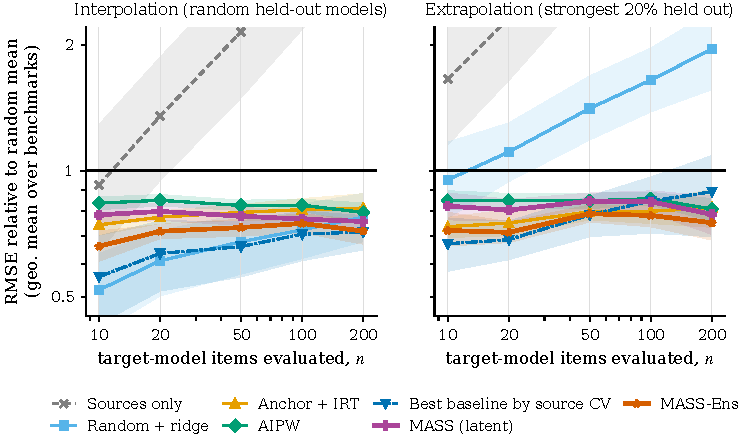
\includegraphics[width=\linewidth]{budget_relrmse.pdf}
\caption{RMSE relative to the random-subset mean as a function of the number of target items, geometric mean over the 13 benchmarks, bands = benchmark-level 95\% intervals. Left: interpolation; right: extrapolation. ``Best baseline by source CV'' selects, per benchmark, the baseline with the lowest RMSE in cross-validation on source models only.}
\label{fig:budget}
\end{figure}

\paragraph{Pre-declared headline (H-main).}
Figure~\ref{fig:paired} gives the paired comparison fixed before the final sweep, at $n\in\{50,100\}$. Under extrapolation, \mass{}-Ens versus random${}+{}$ridge has RMSE ratio 0.56 [0.48, 0.66] ($n=50$) and 0.48 [0.41, 0.56] ($n=100$); versus the baseline with the lowest source-only cross-validated RMSE it has 1.01 [0.93, 1.10] and 0.92 [0.83, 1.05]. The intervals contain 1, so \mass{}-Ens is \emph{not} distinguishable from the best source-CV baseline. The source-CV choice itself is heterogeneous under extrapolation (Anchor Points on 3 benchmarks, anchor-IRT on 3, ridge on 2, information-selected IRT on 2, three other baselines on one each), and picks ridge on GPQA and MuSR, where ridge is indeed below the random mean under extrapolation (RMSE ratios 0.87 and 0.82 at $n=50$; on the ten other benchmarks except LegalBench, ridge is above it, 1.14--2.32). Under interpolation, versus ridge the ratios are 1.08 [0.93, 1.29] and 1.04 [0.91, 1.19], and versus the source-CV choice 1.11 [0.97, 1.31] and 1.06 [0.93, 1.22]: no advantage for \mass{}-Ens, and ridge on the subset is the best point estimate (Table~\ref{tab:head-random}).
At small budgets the point estimate favours the baseline: versus the source-CV choice \mass{}-Ens has ratio 1.08 [0.96, 1.21] at $n=10$ and 1.04 [0.94, 1.14] at $n=20$ under extrapolation (1.18 [0.98, 1.47] and 1.13 [0.95, 1.38] under interpolation); the intervals include 1, and the ratio falls below 1 only from $n=100$ (0.92 [0.83, 1.05]) and $n=200$ (0.84 [0.72, 1.02]), again with intervals that include 1.

\begin{figure}[t]
\centering
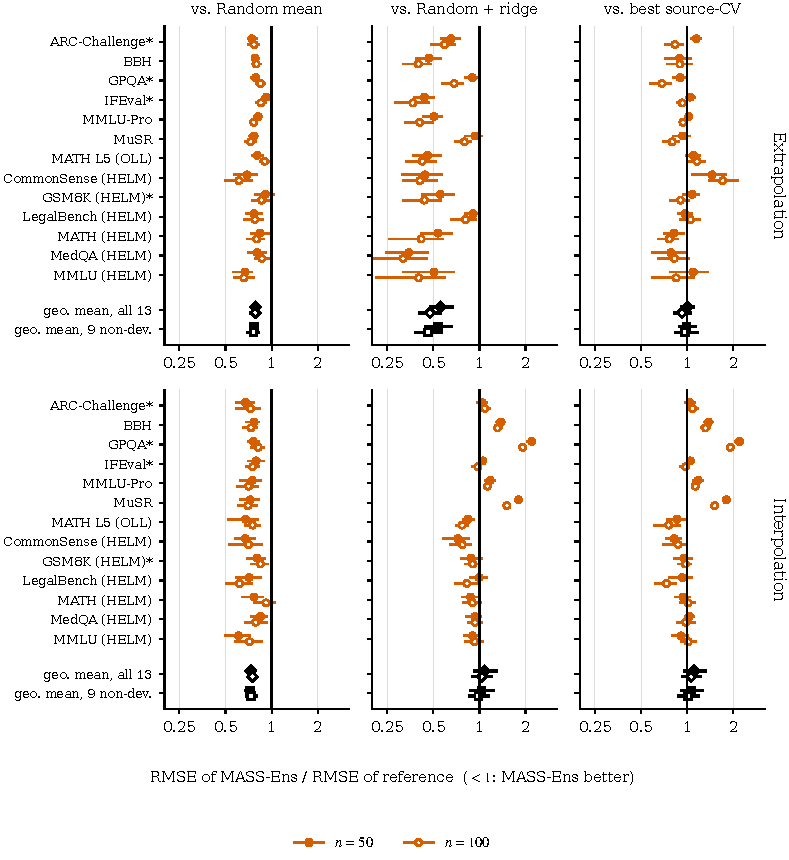
\includegraphics[width=\linewidth]{paired_rmse_mass_ens.pdf}
\caption{Pre-declared comparison. Per benchmark, RMSE(\mass{}-Ens)/RMSE(reference) with paired model-level (extrapolation) or repetition-level (interpolation) 95\% intervals, for $n=50$ (filled) and $n=100$ (open); values below 1 favour \mass{}-Ens. Bottom rows: geometric mean over all 13 benchmarks and over the nine non-development ones. The latent-only \mass{} is in Figure~\ref{fig:paired-mass} (Appendix).}
\label{fig:paired}
\end{figure}

\paragraph{Q3: when do methods fail? Extrapolation and the sign of the error.}
Figure~\ref{fig:scatter} shows true versus predicted scores for three benchmarks under extrapolation. Each point averages the predictions of 20 item-selection seeds, so the panels show the systematic part (bias) of each method, not the error of a single run; the printed RMSE is the per-run RMSE of the tables, not that of the plotted averages. Random${}+{}$ridge is biased low for target models above the source range (median over benchmarks of the mean signed error at $n=50$: $-0.058$; random mean $-0.001$, \mass{}-Ens $-0.008$), flattening toward the source mean, and its RMSE ratio to the random mean is 1.41 [1.18, 1.68] (1.65 at $n=100$). Anchor Points ($-0.026$) and calibration ($-0.036$) show smaller negative biases and ratios of 1.03 [0.80, 1.31] and 1.05 [0.97, 1.14]. The ablations (Table~\ref{tab:ablate}) identify the cause of the safety of \mass{}: with the predictor alone and no difference correction (\texttt{mass\_ens\_nocorr}), the ratio is 1.64 [1.31, 2.03] at $n=100$, i.e.\ it inherits the ridge-like bias, whereas the same predictor with the correction gives 0.78. The correction, not the design or the predictor, keeps the estimator from degrading under extrapolation. The design alone (stratified${}+{}$PPS, Hajek mean) gives 0.86 [0.81, 0.90] and the predictor with correction on random items 0.84 [0.81, 0.87], so each of the three components contributes a little and their combination the most (0.78 [0.74, 0.83]).

\begin{figure}[t]
\centering
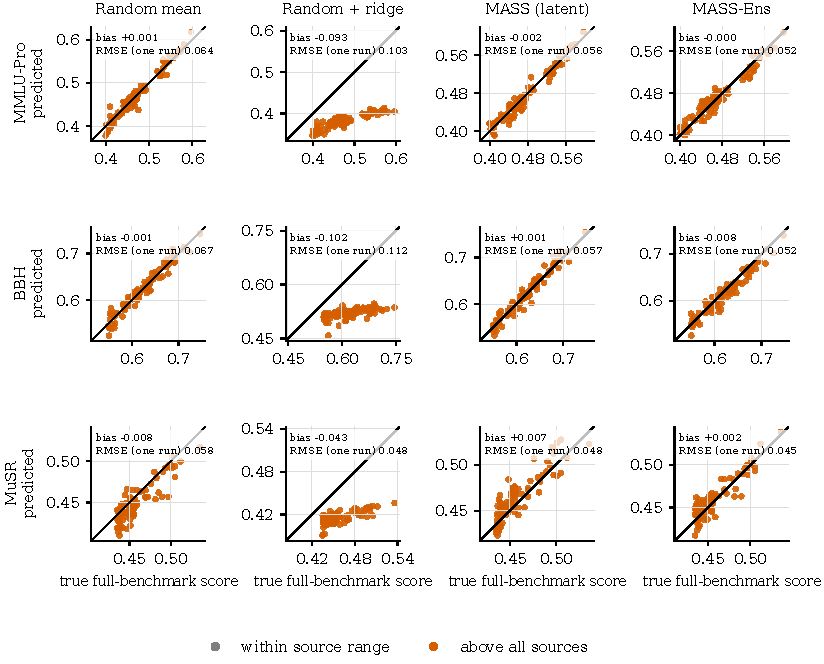
\includegraphics[width=\linewidth]{extrap_scatter.pdf}
\caption{Extrapolation, $n=50$: true versus predicted full-benchmark score of each target model (average over 20 item-selection seeds) for three benchmarks and four methods; points above the source range are orange. Points are averages over seeds and show the systematic part of the error (bias); the printed RMSE is the per-run RMSE of the tables (fractions, not points).}
\label{fig:scatter}
\end{figure}

\begin{table}[t]
\caption{Selection $\times$ prediction under extrapolation and interpolation, $n=100$, RMSE ratio to the random-subset mean, geometric mean over benchmarks (10 repetitions; benchmark-level 95\% intervals). Columns: predictor; ``corr.'' = difference correction on the sample.}
\label{tab:ablate}
\centering\scriptsize
\begin{tabular}{llcccc}
\toprule
Protocol & Design & sample mean & latent + corr. & ensemble + corr. & ensemble, no corr. \\
\midrule
Extrapolation & Random items & 1.00 [1.00, 1.00] & 0.86 [0.83, 0.89] & 0.84 [0.81, 0.87] & 1.67 [1.33, 2.09] \\
 & Stratified & 0.87 [0.84, 0.91] & 0.83 [0.79, 0.89] & -- & -- \\
 & PPS only & -- & 0.81 [0.76, 0.87] & -- & -- \\
 & Stratified + PPS (MASS design) & 0.86 [0.81, 0.90] & 0.84 [0.79, 0.90] & 0.78 [0.74, 0.83] & 1.64 [1.31, 2.03] \\
\midrule
Interpolation & Random items & 1.00 [1.00, 1.00] & 0.83 [0.80, 0.86] & 0.80 [0.77, 0.83] & 0.87 [0.72, 1.05] \\
 & Stratified & 0.84 [0.82, 0.87] & 0.81 [0.79, 0.84] & -- & -- \\
 & PPS only & -- & 0.77 [0.74, 0.80] & -- & -- \\
 & Stratified + PPS (MASS design) & 0.83 [0.79, 0.86] & 0.77 [0.74, 0.80] & 0.75 [0.71, 0.79] & 0.82 [0.69, 0.99] \\
\bottomrule
\end{tabular}

\end{table}

\paragraph{Error is not ranking.}
Lower RMSE does not translate into better ranking of the targets. Under extrapolation the Kendall $\tau_b$ of \mass{}-Ens is 0.46 [0.40, 0.53] against 0.47 [0.40, 0.55] for the random mean at $n=50$ (paired difference $-0.010$ [$-0.040$, $0.037$]); random${}+{}$ridge falls to 0.33 (difference $-0.140$ [$-0.192$, $-0.093$]). Under interpolation \mass{}-Ens improves $\tau_b$ by $0.013$ [$0.003$, $0.025$]. A further reason is spread: with strong models as targets, the median over benchmarks of RMSE divided by the standard deviation of the true target scores is 1.11 for \mass{}-Ens (1.42 for the random mean) under extrapolation, against 0.33 (0.46) under interpolation: the errors are as large as the differences between the models one wants to rank. On the low-spread benchmarks (GPQA, MuSR, MATH Lvl~5) rankings are no better than with the random mean (e.g.\ $\tau_b$ at $n=50$ for GPQA/MuSR: 0.29/0.27 for \mass{}-Ens and 0.29/0.27 for the random mean under extrapolation).

\paragraph{Effective sample size and budget.}
Defining the gain as $(\mathrm{RMSE}_{\text{random}}/\mathrm{RMSE}_{\text{method}})^2$ at equal $n$, the median over benchmarks for \mass{}-Ens is 1.6 at $n=50$ (smallest benchmark 1.17) under extrapolation and 1.8 (smallest 1.40) under interpolation (Figure~\ref{fig:ess}, Appendix): the method is worth roughly 60--80\% more random items, not an order of magnitude. This is the practical size of the effect.

\paragraph{Does the reported uncertainty hold?}
\mass{}-Ens reports a standard error. Averaged over benchmarks, the nominal 95\% interval covers the true target score for 74\% (interpolation: 77\%) of targets at $n=10$, 87\% at $n=20$, 93\% at $n=50$ (extrapolation) and 92\% (interpolation), 95--96\% at $n=100$ and 97\% at $n=200$ (Figure~\ref{fig:cov}, Appendix). It under-covers for $n\le20$, plausibly because the predictor is fit on the sampled items and the standard error ignores this (Section~\ref{sec:mass}), which we did not test separately; we therefore do not claim valid intervals at small $n$.

\paragraph{Q3: sensitivity.}
Table~\ref{tab:robust} and Figure~\ref{fig:sens} (Appendix) vary what the protocol fixes. Holding out whole organisations (a coarse family split) behaves like interpolation: ridge again has the lower point estimate (0.66 [0.54, 0.80] versus 0.75 [0.71, 0.79] for \mass{}-Ens; the intervals overlap) on the seven Open LLM benchmarks. With fewer source models or a larger held-out fraction, ridge degrades visibly under extrapolation while the correction-based estimators change little. Keeping duplicate model rows moves extrapolation ratios (\mass{}-Ens 0.78 to 0.86, AIPW 0.86 to 0.90) while leaving their ordering with respect to ridge unchanged, so duplicate removal matters for the magnitude of the reported gains.

\begin{table}[t]
\caption{Robustness of RMSE ratio to the random mean ($n=100$, 10 repetitions, geometric mean over the benchmarks run). ``dups kept'': exact duplicate model rows not removed. Family-out: Open LLM benchmarks only.}
\label{tab:robust}
\centering\scriptsize
\resizebox{\linewidth}{!}{\begin{tabular}{lccccc}
\toprule
Method & Random (13) & Random, dups kept (13) & Family-out (7) & Extrap. (13) & Extrap., dups kept (13) \\
\midrule
Sources only & 3.13 [2.17, 4.36] & 3.26 [2.25, 4.59] & 2.34 [1.46, 3.69] & 5.63 [3.92, 7.99] & 5.90 [4.07, 8.43] \\
Random + ridge & 0.72 [0.62, 0.83] & 0.74 [0.63, 0.86] & 0.66 [0.54, 0.80] & 1.65 [1.38, 1.96] & 1.69 [1.42, 1.99] \\
Anchor + IRT & 0.81 [0.76, 0.86] & 0.83 [0.78, 0.89] & 0.79 [0.73, 0.84] & 0.80 [0.75, 0.84] & 0.85 [0.81, 0.89] \\
AIPW & 0.83 [0.80, 0.86] & 0.85 [0.82, 0.87] & 0.83 [0.79, 0.87] & 0.86 [0.83, 0.89] & 0.90 [0.87, 0.93] \\
AIPW-Ens & 0.80 [0.77, 0.83] & 0.81 [0.78, 0.84] & 0.80 [0.76, 0.84] & 0.84 [0.81, 0.87] & 0.88 [0.84, 0.92] \\
MASS (latent) & 0.77 [0.74, 0.80] & 0.78 [0.75, 0.82] & 0.79 [0.74, 0.84] & 0.84 [0.79, 0.90] & 0.85 [0.79, 0.91] \\
MASS-Ens & 0.75 [0.71, 0.79] & 0.75 [0.72, 0.79] & 0.75 [0.71, 0.79] & 0.78 [0.74, 0.83] & 0.86 [0.80, 0.92] \\
\bottomrule
\end{tabular}
}
\end{table}

\paragraph{Prior-work hypotheses.}
The code repository of \citet{zhang2025benchmark} states three conclusions, which we treated as hypotheses. (i) \emph{Random sampling plus regression is a strong baseline}: confirmed under interpolation (ridge has the best point estimate, ratio 0.68 at $n=50$) and refuted under extrapolation (1.41). (ii) \emph{Methods degrade when targets exceed the source models}: confirmed for ridge, and mildly for Anchor Points and calibration; qualified for estimators with a difference correction on the sample, which stay below the random mean's RMSE (0.79--0.85) but do not improve ranking. (iii) \emph{AIPW-type estimators help}: confirmed for RMSE against the random mean (13/13 benchmarks) with a latent-trait predictor; with a ridge predictor and cross-fitted residuals the ratio is 0.95 [0.89, 1.03], so the benefit depends on the predictor.
